\documentclass[12pt,a4paper]{article}
\usepackage[UTF8]{ctex}
\usepackage{amsmath,amssymb}
\usepackage{xcolor}
\usepackage{hyperref}
\usepackage{geometry}
\usepackage{graphicx}
\geometry{margin=2.5cm}

\title{Mark State / 标记态}
\author{QuoNic}
\date{}

\begin{document}
\maketitle

\begin{center}
\textbf{Algorithms / 算法} | 难度：初级 | 预计时间：5 分钟
\end{center}

\tableofcontents
\newpage

\section{为什么需要？}

标记态用于标记量子态，是 Grover 搜索的组件。

\subsection{经典局限}
\begin{itemize}
  \item 经典方法无法直接标记量子态
  \item 需要量子标记
\end{itemize}

\subsection{量子优势}
\begin{itemize}
  \item 标记态可以高效标记目标量子态
  \item 是 Grover 搜索的核心组件
  \item 可以自动从经典函数构造
\end{itemize}

\subsection{实际应用}
\begin{itemize}
  \item Grover 搜索
  \item 振幅放大
  \item 量子算法设计
\end{itemize}

\section{快速上手}

\begin{verbatim}
from quonic.algorithms import mark_state

# 标记态
result = mark_state(target='11', n_qubits=2)
print(f'Marked state: {result.state}')
\end{verbatim}

\textbf{预期输出}：
\begin{verbatim}
Marked state: |11>
\end{verbatim}

\section{原理详解}

\subsection{电路图}

\begin{center}
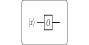
\includegraphics[width=0.6\textwidth]{../../images/mark_state_circuit.svg}
\end{center}

\subsection{数学推导}

标记态：
\begin{equation}
O|x\rangle = (-1)^{f(x)}|x\rangle
\end{equation}

其中 $f(x) = 1$ 当 $x$ 是目标态。

\subsection{几何解释}

标记态在 Bloch 球上翻转目标态的相位。

\section{代码详解}

\begin{verbatim}
from quonic.algorithms import mark_state

# mark_state(target, n_qubits)
# target: 目标态
# n_qubits: 量子比特数

result = mark_state(target='11', n_qubits=2)

# result.state: 标记后的态
# result.oracle: Oracle 矩阵
print(f'Marked state: {result.state}')
\end{verbatim}

\section{进阶用法}

\subsection{场景 1：不同目标态}

\begin{verbatim}
from quonic.algorithms import mark_state

# 不同目标态
r1 = mark_state(target='00', n_qubits=2)
r2 = mark_state(target='11', n_qubits=2)
r3 = mark_state(target='101', n_qubits=3)
\end{verbatim}

\section{适用场景}

\subsection{Grover 搜索}

标记态是 Grover 搜索的核心组件。标记态标记目标态，Diffusion 算子放大目标态的振幅。

\subsection{量子算法设计}

标记态是许多量子算法的基础。例如，振幅放大、量子计数等都需要标记态。

\section{常见问题}

\subsection{标记态和 Oracle 有什么区别？}

标记态是 Oracle 的简化版本。标记态只标记一个目标态，Oracle 可以标记多个目标态。

\subsection{如何构造标记态？}

标记态可以从经典函数自动构造。QuoNic 提供了 mark\_state() 函数来自动构造标记态。

\section{学习路径}

\subsection{前置知识}
\begin{itemize}
  \item 量子门
  \item 量子态
  \item 量子测量
\end{itemize}

\subsection{继续学习}
\begin{itemize}
  \item Grover 搜索
  \item 振幅放大
  \item 量子算法设计
\end{itemize}

\section{完整示例代码}

\subsection{示例 1：基本标记态}

\begin{verbatim}
from quonic.algorithms import mark_state

result = mark_state(target='11', n_qubits=2)
print(f'Marked state: {result.state}')
\end{verbatim}

\section{下载}

\begin{itemize}
  \item [mark\_state.py](https://github.com/ChrisLee0721/QuoNic/blob/main/examples/mark_state/mark_state.py)
\end{itemize}

\end{document}
